\chapter{Oppervlakken, adsorptie en heterogene katalyse}\label{ch:b3:surfaces-catalysis}

Onder een auto, in een stalen omhulsel, zit een keramische honingraat
waarvan de duizenden kanalen bekleed zijn met een poreus oxide dat enkele
grammen platina, palladium en rodium bevat. In een fractie van een
seconde verliezen de uitlaatgassen die erdoor stromen het grootste deel
van hun koolstofmonoxide, onverbrande koolwaterstoffen en stikstofoxiden.
In het gas gebeurt niets: elk van deze reacties vindt plaats op het
oppervlak van metaaldeeltjes van enkele nanometer groot. Het grootste
deel van de chemische industrie werkt op dezelfde manier, van de ammoniak
voor kunstmest tot het kraken van aardolie. Dit hoofdstuk beschrijft hoe
moleculen aan oppervlakken blijven kleven, hoeveel van een oppervlak ze
bedekken, hoe oppervlaktereacties verlopen, en hoe een vaste katalysator
gemaakt, gemeten en bekeken wordt.

\begin{recall}
Het deel van jaar~1 definieerde katalysatoren en het verschil tussen
homogene en heterogene katalyse, en beschreef de kubisch vlakgecentreerde
stapeling van metalen. Het deel van jaar~2 definieerde de omzetting, de
selectiviteit en de omzetfrequentie van een katalysator, en het principe
van Le Chatelier.
\Cref{ch:b3:x-ray-diffraction} voerde de \omterm{def:b3:x-ray-diffraction:miller}{millerindices} in,
\cref{ch:b3:rate-theories} de \omterm{thm:b3:rate-theories:eyring}{vergelijking van Eyring} en
\cref{ch:b3:partition-functions} de statistiek van verdelingen.
\end{recall}

\begin{omfigure}
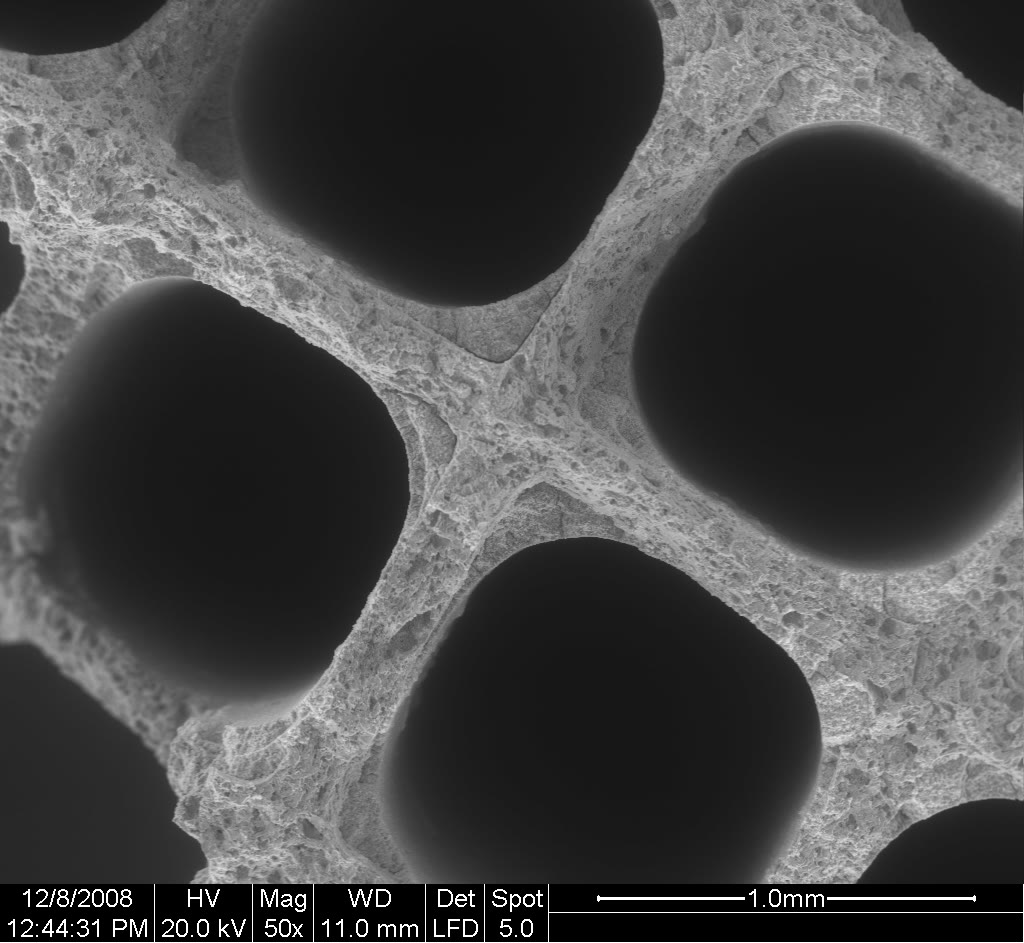
\includegraphics[width=0.48\linewidth]{images/book4/converter-sem.jpg}

{\small De keramische honingraat van een katalysator, gezien met een
rasterelektronenmicroscoop (schaalstreep \qty{1.0}{mm}): vierkante kanalen,
gescheiden door dunne poreuze wanden, die de oxidebekleding en haar
metaaldeeltjes dragen.}
\end{omfigure}

\section{Adsorptie}

\begin{definition}[Adsorptie]\label{def:b3:surfaces-catalysis:adsorption}
\emph{Adsorptie}\index{adsorptie} is de ophoping van moleculen van een gas of
een opgeloste stof op het oppervlak van een vaste stof of een vloeistof.
Het molecuul dat adsorbeert is het
\emph{adsorbaat}\index{adsorbaat}, de vaste stof het
\emph{adsorbens}\index{adsorbens}; het omgekeerde proces is
\emph{desorptie}\index{desorptie}.
\end{definition}

\begin{definition}[Fysisorptie, chemisorptie]\label{def:b3:surfaces-catalysis:physi-chemi}
\emph{Fysisorptie}\index{fysisorptie} is \omterm{def:b3:surfaces-catalysis:adsorption}{adsorptie} door vanderwaalskrachten,
met adsorptie-enthalpieën van hoogstens enkele tientallen kilojoule per
mol, vergelijkbaar met condensatie-enthalpieën, en zonder verandering van
het molecuul. \emph{Chemisorptie}\index{chemisorptie} vormt chemische
bindingen met het oppervlak, met enthalpieën van ongeveer 40 tot enkele
honderden kilojoule per mol; ze kan het molecuul verbreken (dissociatieve
chemisorptie) en stopt bij één laag.
\end{definition}

\begin{omfigure}
\begin{tikzpicture}[font=\small, >=Stealth, x=1cm, y=1cm]
  \draw[->] (0,-2.6) -- (0,1.8) node[anchor=south] {energie};
  \draw[->] (0,0) -- (8.0,0) node[anchor=south east] {afstand tot het oppervlak};
  \draw[omDef, thick] plot[smooth, tension=0.7] coordinates {(1.6,1.6) (2.2,-0.25) (2.8,-0.62) (3.6,-0.35) (5.0,-0.08) (7.5,0)};
  \draw[omThm, thick] plot[smooth, tension=0.6] coordinates {(0.45,1.6) (0.8,-1.2) (1.2,-2.2) (1.7,-1.6) (2.35,-0.15) (2.9,0.9) (3.5,1.5)};
  \node[omDef, anchor=north west, font=\scriptsize] at (3.4,-0.4) {gefysisorbeerd \ce{H2} (precursor)};
  \node[omThm, anchor=west, font=\scriptsize] at (1.75,-1.9) {gechemisorbeerd 2 H};
  \node[omThm, anchor=west, font=\scriptsize, align=left] at (3.55,1.45) {naar $\mathrm{H} + \mathrm{H}$\\ ver van het oppervlak};
  \fill (2.3,-0.2) circle (1.5pt);
  \node[font=\scriptsize] (cr) at (1.25,0.55) {kruising};
  \draw[black!60] (cr.south east) -- (2.27,-0.15);
\end{tikzpicture}

{\small Potentiële energie van een waterstofmolecuul dat een metaaloppervlak
nadert (schematisch). Het molecuul valt eerst in de ondiepe put van de
\omterm{def:b3:surfaces-catalysis:physi-chemi}{fysisorptie}; waar deze kromme de kromme van twee afzonderlijk gebonden
H-atomen kruist, kan het dissociëren in de diepe put van de \omterm{def:b3:surfaces-catalysis:physi-chemi}{chemisorptie}.
Als de kruising boven nul ligt, is de dissociatieve \omterm{def:b3:surfaces-catalysis:physi-chemi}{chemisorptie}
geactiveerd.}
\end{omfigure}

De oppervlakken van metaaldeeltjes vertonen vooral de dichtste vlakken van
het fcc-rooster, (111) en (100). Daarop kan een \omterm{def:b3:surfaces-catalysis:adsorption}{adsorbaat} bovenop één atoom
zitten (topplaats), tussen twee (brugplaats) of in een holte tussen drie
of vier, en de bindingsenergie verschilt van plaats tot plaats.

\begin{omfigure}
\begin{tikzpicture}[font=\scriptsize]
  % fcc(111): hexagonal layer, spacing 0.6 cm
  \foreach \i in {0,...,5}{\foreach \j in {0,...,4}{
    \shade[ball color=black!25] ({0.6*\i+0.3*\j},{0.52*\j}) circle (0.29);}}
  \fill[omThm] (1.2+0.3*1,0.52) circle (0.07);
  \fill[omDef] ({0.6*2+0.3*2+0.3},{0.52*2}) circle (0.07);
  \fill[black] ({0.6*3+0.3*2+0.3},{0.52*2+0.17}) circle (0.07);
  \fill[black!60!green] ({0.6*1+0.3*3+0.3},{0.52*3-0.17}) circle (0.07);
  \node[anchor=north] at (2.1,-0.45) {fcc(111)};
  % fcc(100): square layer
  \begin{scope}[xshift=5.6cm]
  \foreach \i in {0,...,4}{\foreach \j in {0,...,4}{
    \shade[ball color=black!25] ({0.6*\i},{0.6*\j}) circle (0.29);}}
  \fill[omThm] (1.2,1.2) circle (0.07);
  \fill[omDef] (1.5,1.8) circle (0.07);
  \fill[black] (2.1,0.9) circle (0.07);
  \node[anchor=north] at (1.2,-0.45) {fcc(100)};
  \end{scope}
  \node[anchor=west, align=left] at (9.0,1.6) {\textcolor{omThm}{$\bullet$} top\\ \textcolor{omDef}{$\bullet$} brug\\
    $\bullet$ holte (3- of 4-voudig)\\ \textcolor{black!60!green}{$\bullet$} tweede 3-voudige holte (111)};
\end{tikzpicture}

{\small Bovenaanzichten van de twee dichtste vlakken van een kubisch
vlakgecentreerd metaal, met de adsorptieplaatsen: bovenop één atoom,
overbruggend tussen twee, en in de holten tussen drie atomen op (111)
(twee soorten, al dan niet boven een atoom van de tweede laag) of vier
atomen op (100).}
\end{omfigure}

\begin{definition}[Bedekkingsgraad, monolaag]\label{def:b3:surfaces-catalysis:coverage}
De \emph{bedekkingsgraad}\index{bedekkingsgraad} $\theta$ van een oppervlak is
de fractie van zijn adsorptieplaatsen die bezet zijn. Een
\emph{monolaag}\index{monolaag} is één enkele volledige laag \omterm{def:b3:surfaces-catalysis:adsorption}{adsorbaat}, $\theta = 1$.
\end{definition}

\section{Isothermen}

\begin{theorem}[Isotherm van Langmuir]\label{thm:b3:surfaces-catalysis:langmuir}
Als een oppervlak identieke, onafhankelijke plaatsen heeft die elk één
molecuul opnemen, is de \omterm{def:b3:surfaces-catalysis:coverage}{bedekkingsgraad} in evenwicht met een gas bij druk
$p$
\[
  \theta = \frac{Kp}{1 + Kp},
\]
waarin $K$, de adsorptie-evenwichtsconstante, alleen van de temperatuur
afhangt. Dit is de \emph{isotherm van Langmuir}\index{isotherm van Langmuir}.
\end{theorem}

\begin{proof}
Kinetisch bewijs. Moleculen adsorberen op de vrije plaatsen met de snelheid $k_ap(1 - \theta)N$ ($N$
plaatsen) en desorberen met de snelheid $k_d\theta N$. In evenwicht zijn
beide gelijk: $\theta/(1 - \theta)
= (k_a/k_d)p$, wat herschikt het resultaat geeft met $K = k_a/k_d$.

Statistisch bewijs. $M$ moleculen op $N$ plaatsen kunnen op $N!/(M!(N - M)!)$
manieren geschikt worden, waarbij elk geadsorbeerd molecuul een inwendige
toestandssom $q_{\mathrm s}$ heeft (zijn vibraties tegen het oppervlak en
zijn bindingsenergie). Met de formule van Stirling is de chemische
potentiaal van de geadsorbeerde moleculen $\mu_{\mathrm s} = -kT\ln\bigl(q_{\mathrm s}\frac{1 - \theta}{\theta}\bigr)$;
die van het ideale gas is $\mu_{\mathrm g} = \mu_{\mathrm g}^\circ + kT\ln(p/p^\circ)$. Het evenwicht, $\mu_{\mathrm s} = \mu_{\mathrm g}$, geeft
$\theta/(1 - \theta) = q_{\mathrm s}\eu^{\mu_{\mathrm g}^\circ/kT}p/p^\circ$: dezelfde wet, met $K$
uitgedrukt in toestandssommen.
\end{proof}

Bij lage druk is $\theta \approx Kp$ (het henrygebied); bij hoge druk gaat
$\theta \to 1$. De \omterm{def:b3:surfaces-catalysis:coverage}{bedekkingsgraad} is de helft bij $p = 1/K$.

\begin{proposition}[Dissociatieve adsorptie]\label{prop:b3:surfaces-catalysis:dissociative}
Voor een diatomisch gas dat op twee plaatsen dissocieert, $\mathrm{H_2} + 2\,{*} \to 2\,\mathrm{H}{*}$ (${*}$: een vrije plaats), is
\[
  \theta = \frac{(Kp)^{1/2}}{1 + (Kp)^{1/2}},
\]
zodat $\theta \propto \sqrt p$ bij lage druk.
\end{proposition}

\begin{proof}
\omterm{def:b3:surfaces-catalysis:adsorption}{Adsorptie} vereist twee vrije plaatsen, met de snelheid $k_ap(1 - \theta)^2$;
\omterm{def:b3:surfaces-catalysis:adsorption}{desorptie} vereist dat twee geadsorbeerde atomen recombineren, met de
snelheid $k_d\theta^2$. Gelijkheid geeft $\theta/(1 - \theta) =
(Kp)^{1/2}$.
\end{proof}

\begin{proposition}[Competitieve adsorptie]\label{prop:b3:surfaces-catalysis:competitive}
Twee gassen A en B die om dezelfde plaatsen concurreren, bedekken die met
\[
  \theta_{\mathrm A} = \frac{K_{\mathrm A}p_{\mathrm A}}{1 + K_{\mathrm A}p_{\mathrm A} + K_{\mathrm B}p_{\mathrm B}}, \qquad
  \theta_{\mathrm B} = \frac{K_{\mathrm B}p_{\mathrm B}}{1 + K_{\mathrm A}p_{\mathrm A} + K_{\mathrm B}p_{\mathrm B}} .
\]
\end{proposition}

\begin{proof}
Voor elk gas is $k_{a,\mathrm A}p_{\mathrm A}(1 - \theta_{\mathrm A} - \theta_{\mathrm B}) = k_{d,\mathrm A}\theta_{\mathrm A}$, en evenzo voor B. Dus
$\theta_{\mathrm A} = K_{\mathrm A}p_{\mathrm A}\theta_\ast$ en $\theta_{\mathrm B} = K_{\mathrm B}p_{\mathrm B}\theta_\ast$ met $\theta_\ast = 1 - \theta_{\mathrm A} - \theta_{\mathrm B}$ de vrije fractie; optellen
geeft
$1 - \theta_\ast = \theta_\ast(K_{\mathrm A}p_{\mathrm A} + K_{\mathrm B}p_{\mathrm B})$.
\end{proof}

\begin{definition}[Isostere adsorptie-enthalpie]\label{def:b3:surfaces-catalysis:isosteric}
De \emph{isostere adsorptie-enthalpie}\index{isostere adsorptie-enthalpie}
$\Delta_{\mathrm{ads}}H$ is de molaire adsorptie-enthalpie bij een vaste
\omterm{def:b3:surfaces-catalysis:coverage}{bedekkingsgraad}, verkregen uit de drukken die bij verschillende
temperaturen dezelfde \omterm{def:b3:surfaces-catalysis:coverage}{bedekkingsgraad} geven.
\end{definition}

\begin{proposition}[Isostere enthalpie]\label{prop:b3:surfaces-catalysis:isosteric}
Bij constante \omterm{def:b3:surfaces-catalysis:coverage}{bedekkingsgraad} is
\[
  \Bigl(\frac{\partial\ln p}{\partial T}\Bigr)_\theta = -\frac{\Delta_{\mathrm{ads}}H}{RT^2} .
\]
\end{proposition}

\begin{proof}
Bij constante $\theta$ is $Kp$ constant (voor een langmuiroppervlak; in het
algemeen geldt hetzelfde argument met de evenwichtsconstante bij die
\omterm{def:b3:surfaces-catalysis:coverage}{bedekkingsgraad}), dus $\ln p =
\text{constante} - \ln K$. Volgens de vergelijking van Van 't Hoff is $\dd\ln K/\dd T = \Delta_{\mathrm{ads}}H/RT^2$ (met $K$
betrokken op een standaarddruk).
\end{proof}

Omdat \omterm{def:b3:surfaces-catalysis:adsorption}{adsorptie} exotherm is, zijn bij hogere temperaturen hogere drukken
nodig voor dezelfde \omterm{def:b3:surfaces-catalysis:coverage}{bedekkingsgraad}: de isothermen van de figuur dalen
naarmate $T$ stijgt.

\begin{theorem}[BET-isotherm]\label{thm:b3:surfaces-catalysis:bet}
Als moleculen in opeenvolgende lagen adsorberen, de eerste met een
bindingsconstante die kenmerkend is voor het oppervlak en de andere met
het condensatie-evenwicht van de vloeistof, is de geadsorbeerde
hoeveelheid bij relatieve druk $x = p/p^*$ ($p^*$: dampdruk van het
vloeibare \omterm{def:b3:surfaces-catalysis:adsorption}{adsorbaat})
\[
  \frac{v}{v_{\mathrm m}} = \frac{cx}{(1 - x)(1 - x + cx)},
\]
waarin $v_{\mathrm m}$ de hoeveelheid in een \omterm{def:b3:surfaces-catalysis:coverage}{monolaag} is en $c$ een
constante die samenhangt met het verschil tussen de adsorptie-enthalpie in
de eerste laag en de condensatie-enthalpie. Dit is de
\emph{BET-isotherm}\index{BET-isotherm} (Brunauer, Emmett en Teller).
\end{theorem}

\begin{proof}
Zij $s_i$ de fractie van het oppervlak die door precies $i$ lagen bedekt is.
De balans van elke laag geeft, zoals in het bewijs van Langmuir, $s_1 = cxs_0$ en $s_i =
xs_{i-1}$ voor $i \ge 2$, dus $s_i = cx^is_0$. De geadsorbeerde hoeveelheid is $v/v_{\mathrm m} =
\sum_iis_i/\sum_is_i$. Met $\sum_{i\ge1}x^i = x/(1 - x)$ en $\sum_{i\ge1}ix^i = x/(1 - x)^2$:
\[
  \frac{v}{v_{\mathrm m}} = \frac{cs_0\,x/(1 - x)^2}{s_0[1 + cx/(1 - x)]} = \frac{cx}{(1 - x)(1 - x + cx)} .
\]
\end{proof}

Herschikt is $\dfrac{x}{v(1 - x)} = \dfrac{1}{v_{\mathrm m}c} + \dfrac{c - 1}{v_{\mathrm m}c}\,x$: een
rechte waarvan helling en afsnijding $v_{\mathrm m}$ en $c$ geven,
meestal geldig voor $0.05 < x < 0.30$.

\begin{definition}[Specifiek oppervlak]\label{def:b3:surfaces-catalysis:surface-area}
Het \emph{specifiek oppervlak}\index{specifiek oppervlak} van een vaste stof
is haar oppervlakte per massa-eenheid, de wanden van haar poriën
inbegrepen.
\end{definition}

\begin{method}[Specifiek oppervlak uit een stikstofisotherm]\label{met:b3:surfaces-catalysis:bet-area}
\begin{enumerate}
  \item Ontgas het monster onder vacuüm terwijl je het verwarmt; koel het in
        vloeibare stikstof (\qty{77}{K}).
  \item Meet het volume geadsorbeerde stikstof (herleid tot
        standaardomstandigheden) bij relatieve drukken tussen 0.05 en 0.30.
  \item Zet $x/(v(1 - x))$ uit tegen $x$; uit helling en afsnijding volgt
        $v_{\mathrm m} = 1/(\text{helling} + \text{afsnijding})$ en $c = 1 + \text{helling}/\text{afsnijding}$.
  \item Oppervlakte $= n_{\mathrm m}N_Aa_{\mathrm m}$, met $n_{\mathrm m}$ de
        hoeveelheid in de \omterm{def:b3:surfaces-catalysis:coverage}{monolaag} en $a_{\mathrm m} = \qty{0.162}{nm^2}$
        de conventionele oppervlakte van een geadsorbeerd stikstofmolecuul.
\end{enumerate}
\end{method}

\begin{omfigure}
\begin{tikzpicture}
\begin{axis}[name=la, width=0.31\linewidth, height=5.0cm, xmin=0, xmax=100, ymin=0, ymax=1.05,
  axis lines=left, xlabel={$p$ / kPa}, ylabel={$\theta$}, tick label style={font=\small},
  label style={font=\small}, title={\small Langmuir}]
\addplot[omDef, thick] table[x=p_kPa, y=T300] {figdata/out/bachelor-3-langmuir-bet-langmuir.dat};
\addplot[omThm, thick] table[x=p_kPa, y=T350] {figdata/out/bachelor-3-langmuir-bet-langmuir.dat};
\node[font=\scriptsize, omDef, anchor=south east] at (axis cs:98,0.92) {\qty{300}{K}};
\node[font=\scriptsize, omThm, anchor=north east] at (axis cs:98,0.45) {\qty{350}{K}};
\end{axis}
\begin{axis}[name=be, at={(la.east)}, anchor=west, xshift=1.9cm, width=0.31\linewidth, height=5.0cm,
  xmin=0, xmax=0.9, ymin=0, ymax=200, axis lines=left, xlabel={$p/p^*$},
  ylabel={$v$ / \unit{cm^3.g^{-1}}}, tick label style={font=\small}, label style={font=\small},
  title={\small BET}]
\addplot[black, thick] table[x=x, y=v] {figdata/out/bachelor-3-langmuir-bet-bet.dat};
\addplot[only marks, mark=*, mark size=1.4pt, omDef] table[x=x, y=v] {figdata/out/bachelor-3-langmuir-bet-data.dat};
\draw[black!40, dashed] (axis cs:0,45) -- (axis cs:0.9,45);
\node[font=\scriptsize, anchor=south east] at (axis cs:0.88,45) {$v_{\mathrm m}$};
\end{axis}
\begin{axis}[at={(be.east)}, anchor=west, xshift=2.1cm, width=0.31\linewidth, height=5.0cm,
  xmin=0, xmax=0.35, ymin=0, ymax=0.0085, axis lines=left, xlabel={$x = p/p^*$},
  ylabel={$x/(v(1 - x))$}, tick label style={font=\small}, label style={font=\small},
  scaled y ticks=false, yticklabel style={/pgf/number format/fixed, /pgf/number format/precision=3},
  title={\small BET-grafiek}]
\addplot[black, thin] table[x=x, y=y] {figdata/out/bachelor-3-langmuir-bet-line.dat};
\addplot[only marks, mark=*, mark size=1.4pt, omDef] table[x=x, y=y] {figdata/out/bachelor-3-langmuir-bet-data.dat};
\end{axis}
\end{tikzpicture}

{\small Links: \omterm{thm:b3:surfaces-catalysis:langmuir}{isothermen van Langmuir} van een modelchemisorptie
($\Delta_{\mathrm{ads}}H = \qty{-40}{kJ/mol}$) bij twee temperaturen.
Midden: een \omterm{thm:b3:surfaces-catalysis:bet}{BET-isotherm} (model, $v_{\mathrm m} = \qty{45}{cm^3.g^{-1}}$, $c = 120$), met de
punten van het weekendprobleem; de lagen stapelen zich op en de
hoeveelheid divergeert nabij
$p = p^*$, waar het gas condenseert. Rechts: de lineaire BET-grafiek van
dezelfde punten.}
\end{omfigure}

\section{Kinetiek van oppervlaktereacties}

\begin{definition}[Mechanismen van Langmuir-Hinshelwood en Eley-Rideal]\label{def:b3:surfaces-catalysis:mechanisms}
In het \emph{mechanisme van
Langmuir-Hinshelwood}\index{mechanisme van Langmuir-Hinshelwood} zijn beide
beginstoffen geadsorbeerd en reageren ze op het oppervlak; in het
\emph{mechanisme van Eley-Rideal}\index{mechanisme van Eley-Rideal}
reageert een geadsorbeerde beginstof met een molecuul dat uit het gas
aankomt.
\end{definition}

\begin{proposition}[Snelheid volgens Langmuir-Hinshelwood]\label{prop:b3:surfaces-catalysis:lh-rate}
Als de adsorptie-evenwichten snel zijn en de oppervlaktereactie van
geadsorbeerd A en B snelheidsbepalend is, is
\[
  r = k\theta_{\mathrm A}\theta_{\mathrm B} = \frac{kK_{\mathrm A}p_{\mathrm A}K_{\mathrm B}p_{\mathrm B}}{(1 + K_{\mathrm A}p_{\mathrm A} + K_{\mathrm B}p_{\mathrm B})^2},
\]
wat, bij vaste $p_{\mathrm B}$, het grootst is wanneer $K_{\mathrm A}p_{\mathrm A} = 1 + K_{\mathrm B}p_{\mathrm B}$ en daarna
daalt naarmate A B van het oppervlak verdringt.
\end{proposition}

\begin{proof}
De bedekkingsgraden zijn die van \cref{prop:b3:surfaces-catalysis:competitive}. Met $u =
K_{\mathrm A}p_{\mathrm A}$ en $a = 1 + K_{\mathrm B}p_{\mathrm B}$ is $r \propto u/(a + u)^2$, waarvan de afgeleide $(a - u)/(a + u)^3$ nul wordt bij
$u = a$.
\end{proof}

\begin{proposition}[Snelheid volgens Eley-Rideal]\label{prop:b3:surfaces-catalysis:er-rate}
Als geadsorbeerd A reageert met gasvormig B, is
\[
  r = k\theta_{\mathrm A}p_{\mathrm B} = \frac{kK_{\mathrm A}p_{\mathrm A}p_{\mathrm B}}{1 + K_{\mathrm A}p_{\mathrm A}},
\]
wat met $p_{\mathrm A}$ groeit tot een plateau, zonder maximum.
\end{proposition}

\begin{proof}
B concurreert niet om de plaatsen: $\theta_{\mathrm A}$ is de \omterm{def:b3:surfaces-catalysis:coverage}{bedekkingsgraad}
van Langmuir van A alleen, en de snelheid is daarmee evenredig en met de
botsingsfrequentie van B met het oppervlak, die evenredig is met $p_{\mathrm B}$.
\end{proof}

\begin{method}[LH of ER uit de drukafhankelijkheid]\label{met:b3:surfaces-catalysis:mechanism-from-rate}
\begin{enumerate}
  \item Meet de snelheid als functie van de druk van elke beginstof, terwijl
        de andere vast gehouden wordt.
  \item Een maximum, daarna een daling (negatieve orde bij hoge druk):
        Langmuir-Hinshelwood, waarbij de beginstof inhibeert door de
        plaatsen te bezetten.
  \item Een stijging tot een plateau voor de ene beginstof en eerste orde
        voor de andere bij alle drukken: Eley-Rideal.
  \item Bevestig met isotoopmerking of oppervlaktespectroscopie; de meeste
        katalytische reacties blijken van het type Langmuir-Hinshelwood te
        zijn.
\end{enumerate}
\end{method}

\begin{omfigure}
\begin{tikzpicture}
\begin{axis}[width=0.6\linewidth, height=5.4cm, xmin=0, xmax=10, ymin=0, ymax=0.3,
  axis lines=left, xlabel={$p_{\mathrm A}$ (gereduceerd)}, ylabel={snelheid (gereduceerd)},
  tick label style={font=\small}, label style={font=\small},
  legend style={font=\scriptsize, draw=none, at={(1.03,0.98)}, anchor=north west}, legend cell align=left]
\addplot[omDef!50, thick] table[x=pA, y=pB05] {figdata/out/bachelor-3-surface-rates.dat};
\addplot[omDef, thick] table[x=pA, y=pB1] {figdata/out/bachelor-3-surface-rates.dat};
\addplot[black, thick] table[x=pA, y=pB3] {figdata/out/bachelor-3-surface-rates.dat};
\addplot[omThm, thick, dashed] table[x=pA, y=ER] {figdata/out/bachelor-3-surface-rates.dat};
\legend{{LH, $p_{\mathrm B} = 0.5$}, {LH, $p_{\mathrm B} = 1$}, {LH, $p_{\mathrm B} = 3$}, {ER ($\times\frac14$)}}
\end{axis}
\end{tikzpicture}

{\small Snelheden van een bimoleculaire oppervlaktereactie als functie van
de druk van A (gereduceerde eenheden, $K_{\mathrm A} = K_{\mathrm B} = 1$).
Langmuir-Hinshelwood: elke kromme bereikt een maximum bij $K_{\mathrm A}p_{\mathrm A} =
1 + K_{\mathrm B}p_{\mathrm B}$ en daalt daarna naarmate A B verdringt.
Eley-Rideal (gestreept, geschaald): een plateau.}
\end{omfigure}

\begin{proposition}[Schijnbare activeringsenergie]\label{prop:b3:surfaces-catalysis:apparent-ea}
Voor een monomoleculaire oppervlaktereactie met \omterm{def:b3:surfaces-catalysis:adsorption}{adsorptie} volgens Langmuir
is $r = k\theta = kKp/(1 + Kp)$.
Bij lage \omterm{def:b3:surfaces-catalysis:coverage}{bedekkingsgraad} is de gemeten activeringsenergie $E_{a,\mathrm{app}} = E_a + \Delta_{\mathrm{ads}}H$; bij
hoge \omterm{def:b3:surfaces-catalysis:coverage}{bedekkingsgraad} is ze $E_a$.
\end{proposition}

\begin{proof}
Bij lage \omterm{def:b3:surfaces-catalysis:coverage}{bedekkingsgraad} is $r \approx kKp$, dus $\dd\ln r/\dd T = \dd\ln k/\dd T + \dd\ln K/\dd T = (E_a + \Delta_{\mathrm{ads}}H)/RT^2$.
Bij hoge \omterm{def:b3:surfaces-catalysis:coverage}{bedekkingsgraad} is $\theta \approx 1$ en $r \approx k$.
\end{proof}

Omdat $\Delta_{\mathrm{ads}}H < 0$, lijkt een reactie op een schaars bedekt
oppervlak gemakkelijker dan haar echte barrière: de temperatuur verhogen
versnelt de oppervlaktestap maar maakt het oppervlak leeg.

\begin{definition}[Principe van Sabatier, vulkaangrafiek]\label{def:b3:surfaces-catalysis:sabatier}
Het \emph{principe van Sabatier}\index{principe van Sabatier} stelt dat de
beste katalysator de beginstoffen noch te zwak bindt (ze adsorberen of
activeren niet) noch te sterk (de producten vertrekken niet en blokkeren
de plaatsen). Een
\emph{vulkaangrafiek}\index{vulkaangrafiek} van de activiteit van een reeks
katalysatoren als functie van een bindingsenergie heeft een maximum bij
een gemiddelde binding.
\end{definition}

\begin{omfigure}
\begin{tikzpicture}[font=\small, >=Stealth]
  \draw[->] (0,0) -- (7.2,0) node[anchor=north east] {bindingssterkte van het adsorbaat};
  \draw[->] (0,0) -- (0,3.6) node[anchor=south] {activiteit};
  \draw[omDef, very thick] (0.4,0.3) -- (3.4,3.0) -- (6.6,0.4);
  \node[anchor=south, align=center, font=\scriptsize] at (1.35,2.0) {bindt te zwak:\\ beginstoffen niet\\ geactiveerd};
  \node[anchor=south, align=center, font=\scriptsize] at (5.9,2.0) {bindt te sterk:\\ producten blokkeren\\ de plaatsen};
  \node[anchor=south, font=\scriptsize] at (3.4,3.05) {beste katalysator};
\end{tikzpicture}

{\small Een \omterm{def:b3:surfaces-catalysis:sabatier}{vulkaangrafiek} (kwalitatief): de activiteit van een reeks
katalysatoren als functie van de sterkte waarmee ze een sleutelintermediair
binden.}
\end{omfigure}

\section{Industriële katalysatoren}

\begin{definition}[Opbouw van een katalysator]\label{def:b3:surfaces-catalysis:catalyst-design}
Een \emph{katalysatordrager}\index{katalysatordrager} is een poreuze vaste
stof met een groot oppervlak (aluminiumoxide, siliciumdioxide, koolstof)
die kleine deeltjes van de actieve fase draagt. Een
\emph{promotor}\index{promotor} is een additief, op zich inactief, dat de
activiteit, selectiviteit of stabiliteit verhoogt. Een
\emph{katalysatorgif}\index{katalysatorgif}
is een stof die sterk aan de actieve plaatsen bindt en ze blokkeert.
De \emph{metaaldispersie}\index{metaaldispersie} $D$ is de fractie van de
metaalatomen die aan het oppervlak liggen. \emph{Sinteren}\index{sinteren}
is de groei van de deeltjes bij hoge temperatuur, wat de dispersie
verlaagt.
\end{definition}

\begin{method}[Dispersie en deeltjesgrootte uit waterstofchemisorptie]\label{met:b3:surfaces-catalysis:dispersion}
\begin{enumerate}
  \item Reduceer de katalysator in waterstof, maak vacuüm, en meet het
        volume \ce{H2} dat op het metaal gechemisorbeerd wordt (herleid tot
        standaardomstandigheden); de drager adsorbeert niets.
  \item Neem één H-atoom per metaalatoom aan het oppervlak aan: $D = n_{\ce{H}}/n_{\text{metaal}}$.
  \item Voor bollen met diameter $d$ is $D = 6(v_{\mathrm{at}}/a_{\mathrm{at}})/d$, met $v_{\mathrm{at}}$ het volume per atoom in de
        bulk en $a_{\mathrm{at}}$ de oppervlakte per oppervlakteatoom; dus $d = 6v_{\mathrm{at}}/(a_{\mathrm{at}}D)$.
\end{enumerate}
\end{method}

De ammoniaksynthese, $\ce{N2 + 3 H2 <=> 2 NH3}$, verloopt bij ongeveer 400 tot
\qty{500}{\celsius} en 100 tot \qty{300}{bar} op ijzer, gepromoot met
kaliumoxide en aluminiumoxide: het aluminiumoxide verhindert dat de
ijzerkristallieten \omterm{def:b3:surfaces-catalysis:catalyst-design}{sinteren}, het kalium verhoogt de activiteit. De
snelheidsbepalende stap is de dissociatieve \omterm{def:b3:surfaces-catalysis:physi-chemi}{chemisorptie} van \ce{N2},
waarvan de drievoudige binding het moeilijkst te verbreken is. Zo wordt
er jaarlijks zo'n 150 miljoen ton stikstof vastgelegd.
% ledger: nh3:world-2024
De oxidatie van \ce{SO2} tot \ce{SO3}, op vanadium(V)oxide gepromoot met
kaliumsulfaat, is de sleutelstap van de productie van zwavelzuur.

De driewegkatalysator van benzinemotoren oxideert CO en koolwaterstoffen
en reduceert tegelijk stikstofoxiden, op platina en palladium (oxidatie)
en rodium (reductie van NO), gedispergeerd op aluminiumoxide met
ceriumoxide, dat zuurstof opslaat en vrijgeeft. Hij werkt alleen in een
smal venster rond de stoichiometrische lucht-brandstofverhouding: met
overmaat lucht wordt NO niet gereduceerd, met overmaat brandstof wordt CO
niet geoxideerd; een zuurstofsensor in de uitlaat houdt de motor in het
venster. Lood uit gelode benzine vergiftigt het metaal, wat een van de
redenen is waarom gelode benzine verdween. Zeolieten, kristallijne
aluminosilicaten met poriën van moleculaire grootte en zure plaatsen,
kraken de grote moleculen van zware oliefracties tot benzine en laten
alleen moleculen toe die in hun kanalen passen.

\begin{omfigure}
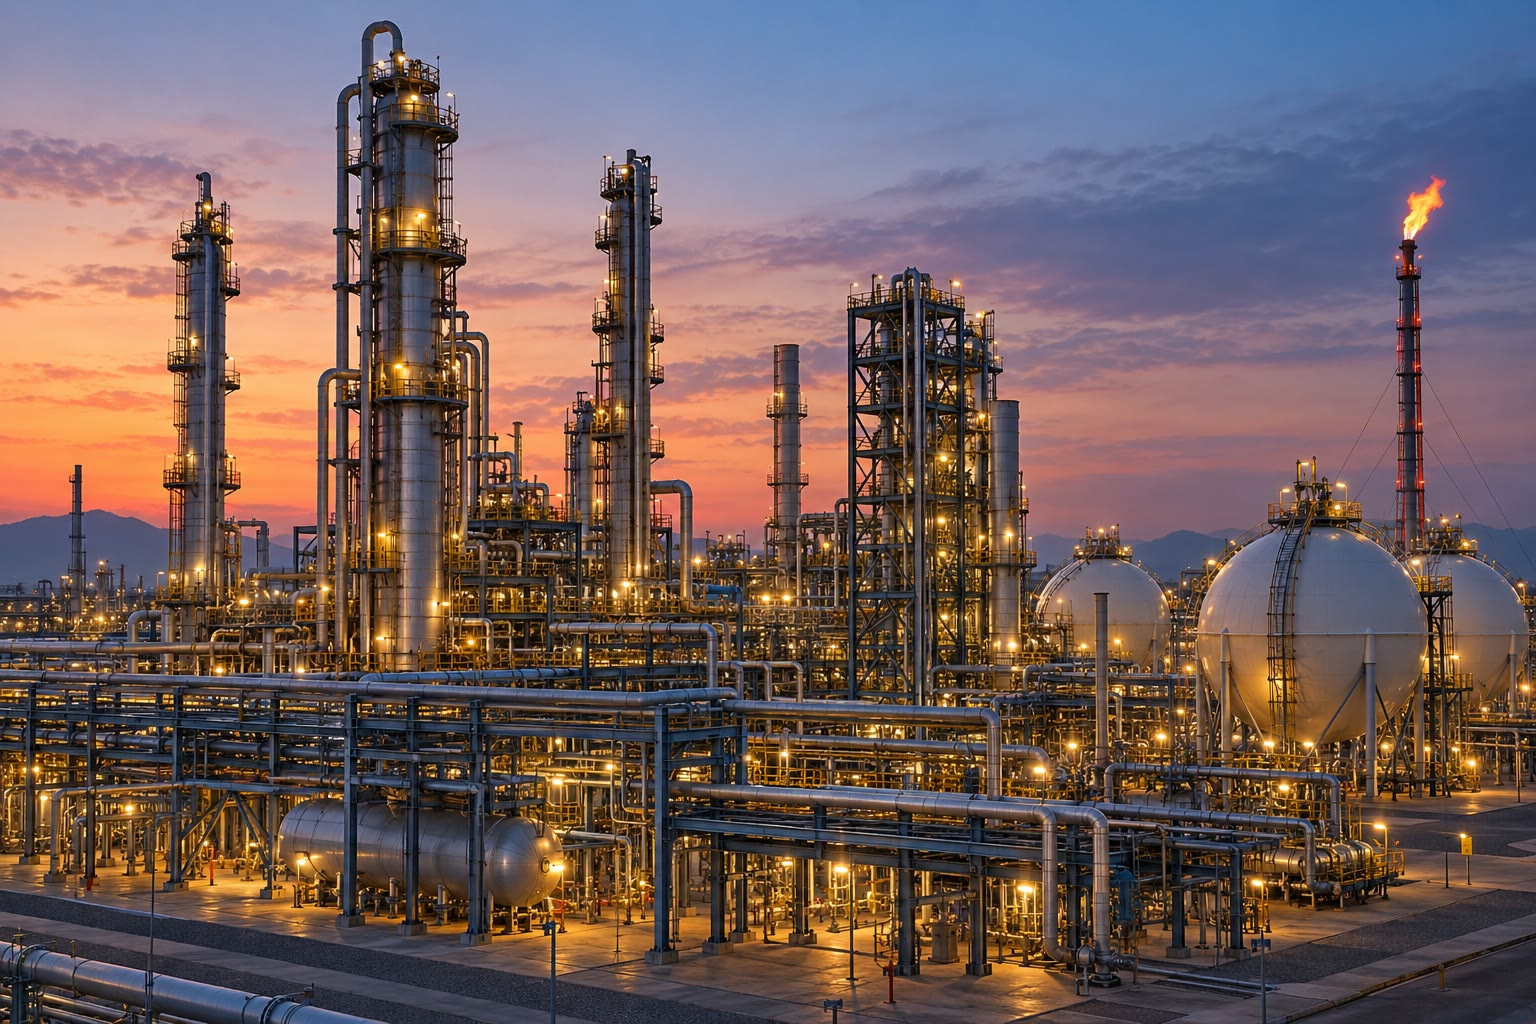
\includegraphics[width=0.6\linewidth]{images/book4/ai/b3-16-ammonia-plant.jpg}

{\small Een fabriek voor ammoniaksynthese. De reactor in het hart ervan
bevat tonnen gepromoot ijzerkatalysator; het grootste deel van de fabriek
bereidt de waterstof en recycleert het niet-omgezette gas.}
\end{omfigure}

\section{Oppervlakken bekijken}

\begin{definition}[Thermische desorptiespectroscopie]\label{def:b3:surfaces-catalysis:tpd}
\emph{Thermische desorptiespectroscopie}\index{thermische desorptiespectroscopie}
verwarmt een oppervlak met een \omterm{def:b3:surfaces-catalysis:adsorption}{adsorbaat} met een constante snelheid en
registreert het desorberende gas met een massaspectrometer; elke
bindingstoestand geeft een piek, waarvan de temperatuur stijgt met haar
desorptieactiveringsenergie.
\end{definition}

De positie van een desorptiepiek geeft de desorptie-energie (voor een
\omterm{def:b3:surfaces-catalysis:adsorption}{desorptie} van de eerste orde is $E_d \approx RT_{\mathrm p}[\ln(\nu T_{\mathrm p}/\beta) - 3.64]$ met $\beta$ de opwarmsnelheid en $\nu \approx \qty{e13}{s^{-1}}$,
hier aangenomen), haar oppervlakte de geadsorbeerde hoeveelheid.
Foto-elektronspectroscopie met röntgenstralen (XPS) meet de
bindingsenergieën van de kernelektronen van de oppervlakteatomen, die de
elementen en hun oxidatietoestanden in de eerste paar nanometer
identificeren. De rastertunnelmicroscoop beweegt een scherpe tip enkele
tienden van een nanometer boven een geleidend oppervlak; de tunnelstroom
(\cref{ch:b3:quantum-model-systems}) daalt met ongeveer een grootteorde
per \qty{0.1}{nm} extra afstand, zodat het constant houden ervan tijdens
het scannen het oppervlak atoom voor atoom in kaart brengt.

\begin{inthelab}[Een BET-meting]
Ongeveer \qty{0.2}{g} monster wordt afgewogen in een glazen buis met een
bol, urenlang ontgast onder vacuüm bij 150 tot \qty{300}{\celsius},
opnieuw gewogen en op het toestel gemonteerd, met de bol ondergedompeld in
een dewarvat met vloeibare stikstof. Het toestel laat stikstof in kleine
doses toe en meet na elke dosis de evenwichtsdruk, waaruit het met een
gasbalans de geadsorbeerde hoeveelheid afleidt; het dode volume van de
buis wordt gemeten met helium, dat niet adsorbeert.
\end{inthelab}

\begin{safety}{\ghs[0.7cm]{GHS06}\ghs[0.7cm]{GHS07}\ghs[0.7cm]{GHS08}\ghs[0.7cm]{GHS09}}
% ledger: ghs4:V2O5, ghs4:Ni
Gereduceerde metaalkatalysatoren (fijnverdeeld nikkel, palladium of
platina op een drager, pas gereduceerd in waterstof) kunnen bij contact
met lucht ontbranden: ze worden onder inert gas gehanteerd en vóór de
opslag gepassiveerd. Nikkel is een huidsensibilisator en verdacht
kankerverwekkend; vanadium(V)oxide is giftig bij inademing en inslikken en
kan kanker veroorzaken. Katalysatorpoeders worden afgewogen in een
geventileerde kast.
\end{safety}

\begin{history}[Langmuir en de ammoniakkatalysator]
Irving Langmuir, die in een industrieel laboratorium aan gloeilampen
werkte, leidde zijn isotherm in 1916--1918 af uit het idee dat
geadsorbeerde gassen een laag van één molecuul dik vormen, en ontving de
Nobelprijs voor de Scheikunde van 1932 voor zijn oppervlaktechemie.
Enkele jaren eerder had Alwin Mittasch de zoektocht naar een bruikbare
ammoniakkatalysator georganiseerd: duizenden samenstellingen werden in
kleine hogedrukreactoren getest voordat de gepromote ijzerkatalysator, die
nog steeds gebruikt wordt, gekozen werd. Het was een van de eerste
systematische screenings van katalysatoren.
\end{history}

\section{Oefeningen}

\begin{exercise}[$\star$]\label{exo:b3:surfaces-catalysis:1}
Een gas bedekt 40\,\% van een langmuiroppervlak bij \qty{2.0}{kPa}. Bereken
$K$ en de \omterm{def:b3:surfaces-catalysis:coverage}{bedekkingsgraad} bij
\qty{10}{kPa}.
\end{exercise}

\begin{exercise}[$\star$]\label{exo:b3:surfaces-catalysis:2}
Op een metaal worden twee adsorptie-enthalpieën gemeten: $-20$ en
\qty{-150}{kJ/mol}. Welke is \omterm{def:b3:surfaces-catalysis:physi-chemi}{fysisorptie}, welke \omterm{def:b3:surfaces-catalysis:physi-chemi}{chemisorptie}? Welke zou
dissociatief kunnen zijn?
\end{exercise}

\begin{exercise}[$\star$]\label{exo:b3:surfaces-catalysis:3}
Tel per oppervlakteatoom de top-, brug- en holteplaatsen van een vlak
(100) en van een vlak (111) van een fcc-metaal.
\end{exercise}

\begin{exercise}[$\star$]\label{exo:b3:surfaces-catalysis:4}
Een katalysator zet \qty{3.0e-6}{mol} beginstof om per gram per seconde en
draagt
\qty{1.5e-5}{mol} oppervlakteplaatsen per gram. Bereken de omzetfrequentie.
\end{exercise}

\begin{exercise}[$\star\star$]\label{exo:b3:surfaces-catalysis:5}
Waterstof adsorbeert dissociatief met $\theta = 0.10$ bij \qty{1.0}{kPa}. Bereken $\theta$ bij \qty{4.0}{kPa}.
\end{exercise}

\begin{exercise}[$\star\star$]\label{exo:b3:surfaces-catalysis:6}
CO ($K = \qty{10}{kPa^{-1}}$) en \ce{O2} ($K = \qty{0.5}{kPa^{-1}}$, in dit eenvoudige model niet dissociatief)
concurreren om de plaatsen van een platinaoppervlak bij 1.0 en
\qty{5.0}{kPa}. Bereken de twee bedekkingsgraden en becommentarieer de
snelheid van de CO-oxidatie.
\end{exercise}

\begin{exercise}[$\star\star$]\label{exo:b3:surfaces-catalysis:7}
Een \omterm{def:b3:surfaces-catalysis:coverage}{bedekkingsgraad} die bij \qty{300}{K} bereikt wordt bij \qty{1.0}{kPa},
vereist bij \qty{350}{K} \qty{8.0}{kPa}. Bereken de \omterm{def:b3:surfaces-catalysis:isosteric}{isostere
adsorptie-enthalpie}.
\end{exercise}

\begin{exercise}[$\star\star$]\label{exo:b3:surfaces-catalysis:8}
% ledger: sa:N2.am, const:Vm1, const:NA
Een actieve kool heeft $v_{\mathrm m} = \qty{120}{cm^3.g^{-1}}$
(standaardomstandigheden, 273.15 K en
\qty{101.325}{kPa}). Bereken haar BET-oppervlak.
\end{exercise}

\begin{exercise}[$\star\star$]\label{exo:b3:surfaces-catalysis:9}
De snelheid van $\ce{2 CO + O2 -> 2 CO2}$ op platina stijgt, bereikt een
maximum en daalt naarmate $p(\ce{CO})$ toeneemt bij vaste $p(\ce{O2})$. Op
welk mechanisme wijst dit, en waarom inhibeert CO de reactie?
\end{exercise}

\begin{exercise}[$\star\star\star$]\label{exo:b3:surfaces-catalysis:10}
Een oppervlaktereactie heeft een echte activeringsenergie van
\qty{100}{kJ/mol}; de beginstof heeft
$\Delta_{\mathrm{ads}}H = \qty{-60}{kJ/mol}$. Welke activeringsenergie wordt
gemeten bij lage en bij hoge \omterm{def:b3:surfaces-catalysis:coverage}{bedekkingsgraad}? Schets $\ln r$ tegen $1/T$
over een breed gebied.
\end{exercise}

\begin{exercise}[$\star\star\star$]\label{exo:b3:surfaces-catalysis:11}
Zwavel adsorbeert op een nikkelkatalysator met een \omterm{def:b3:surfaces-catalysis:coverage}{bedekkingsgraad} van
0.10 (zwavelatomen per Ni-atoom aan het oppervlak), waarbij elk
zwavelatoom vier plaatsen blokkeert. Welke fractie van de activiteit
blijft over voor een reactie die één vrije plaats nodig heeft? En twee
naburige vrije plaatsen (neem aan dat de geblokkeerde plaatsen
willekeurig liggen)?
\end{exercise}

\begin{exercise}[$\star\star\star$]\label{exo:b3:surfaces-catalysis:12}
Voor de ammoniaksynthese binden drie metalen atomaire stikstof met
enthalpieën van
$-150$, $-250$ en \qty{-400}{kJ/mol} (gegevens van de oefening). Welk
metaal is volgens het \omterm{def:b3:surfaces-catalysis:sabatier}{principe van Sabatier} waarschijnlijk de beste
katalysator, en wat beperkt de andere twee?
\end{exercise}

\section{Probleem: een katalysator meten}

\begin{problem}[{Weekendprobleem --- een katalysator meten: het BET-oppervlak
van een platinakatalysator op een drager, zijn metaaldispersie en
deeltjesgrootte uit waterstofchemisorptie, en de omzetfrequentie van een
hydrogenering}]
\label{pb:b3:surfaces-catalysis:1}
% ledger: sa:N2.am, lat:Pt, aw:Pt, const:Vm1, const:NA
Een katalysator bevat 1.00 massaprocent platina op aluminiumoxide.
Gegevens van het probleem: stikstofisotherm bij \qty{77}{K} (volumes bij
standaardomstandigheden, 273.15 K en
\qty{101.325}{kPa}, per gram):
\begin{center}\small
\begin{tabular}{lcccccc}
\hline
$x = p/p^*$ & 0.05 & 0.10 & 0.15 & 0.20 & 0.25 & 0.30 \\
$v$ / \unit{cm^3.g^{-1}} & 41.2 & 46.1 & 51.1 & 54.1 & 58.9 & 62.9 \\ \hline
\end{tabular}
\end{center}
Op het platina gechemisorbeerd \ce{H2}: \qty{0.205}{cm^3} per gram
katalysator. Een hydrogenering
verloopt met \qty{2.0e-5}{mol} per gram katalysator per seconde. Platina: $M = \qty{195.08}{g/mol}$, fcc,
$a = \qty{392.3}{pm}$; molair volume van een gas bij
standaardomstandigheden \qty{22414}{cm^3/mol};
$a_{\mathrm m}(\ce{N2}) = \qty{0.162}{nm^2}$.

\medskip\noindent\textbf{Deel I --- De BET-grafiek.}
\begin{enumerate}
  \item Waarom wordt de isotherm gemeten bij \qty{77}{K}?
  \item Waarom gebruikt men alleen relatieve drukken tussen 0.05 en 0.30?
  \item Bereken $x/(v(1 - x))$ voor elk punt.
  \item De kleinstekwadratenrechte heeft helling \num{0.02205} en afsnijding
        \num{0.000180} (in
        \unit{g.cm^{-3}}). Leid $v_{\mathrm m}$ af.
  \item Leid $c$ af. Wat betekent een grote $c$?
  \item Waarom is de afsnijding zo slecht bepaald, en maakt dat uit voor
        $v_{\mathrm m}$?
\end{enumerate}

\medskip\noindent\textbf{Deel II --- De oppervlakte.}
\begin{enumerate}[resume]
  \item Bereken de hoeveelheid stikstof in de \omterm{def:b3:surfaces-catalysis:coverage}{monolaag} per gram.
  \item Bereken het \omterm{def:b3:surfaces-catalysis:surface-area}{specifiek oppervlak}.
  \item Welk deel van de vaste stof levert bijna al deze oppervlakte?
  \item Waarom faalt de BET-methode voor microporeuze vaste stoffen zoals
        zeolieten?
\end{enumerate}

\medskip\noindent\textbf{Deel III --- Dispersie en deeltjesgrootte.}
\begin{enumerate}[resume]
  \item Bereken de hoeveelheid gechemisorbeerde H-atomen per gram.
  \item Bereken de hoeveelheid platina per gram.
  \item Leid de dispersie af.
  \item Bereken het volume per Pt-atoom in de bulk.
  \item De oppervlakte per oppervlakteatoom, gemiddeld over de vlakken
        (111), (100) en (110), is \qty{0.0807}{nm^2}. Controleer de waarde
        voor (111), $\frac{\sqrt3}{4}a^2$.
  \item Toon aan dat voor bollen $d = 6v_{\mathrm{at}}/(a_{\mathrm{at}}D)$.
  \item Bereken de gemiddelde deeltjesdiameter.
  \item Welke aannamen beperken dit resultaat?
\end{enumerate}

\medskip\noindent\textbf{Deel IV --- Activiteit.}
\begin{enumerate}[resume]
  \item Bereken de omzetfrequentie per Pt-atoom aan het oppervlak.
  \item Bereken de snelheid per gram platina.
  \item Als de deeltjes bij constante omzetfrequentie tot \qty{10}{nm}
        sinterden, met welke factor zou de snelheid per gram dalen?
  \item Wat zou een omzetfrequentie die met de deeltjesgrootte verandert,
        onthullen?
  \item Waarom vergelijkt men katalysatoren met de omzetfrequentie in
        plaats van met de snelheid per gram?
  \item Formuleer het resultaat: de gemiddelde diameter van de
        platinadeeltjes.
\end{enumerate}
\end{problem}
